\title{Introdução às Listas Ligadas}
\date{\today}
\frame{\titlepage}

% Slide 1: Flexibilidade de Memória
\begin{frame}[fragile]
  \frametitle{Flexibilidade de Memória}
  \begin{itemize}
  \item \textbf{Alocação Dinâmica:} Diferentemente dos vetores, que precisam de um tamanho definido na sua criação, listas ligadas permitem alocação dinâmica de memória.
  \item \textbf{Crescimento Incremental:} É possível adicionar novos nós à lista ligada sem a necessidade de realocação ou cópia de dados, ao contrário dos vetores, que podem exigir realocação e cópia de todo o array quando o espaço alocado inicialmente é excedido.
  \item \textbf{Eficiência de Espaço:} Com listas ligadas, a memória é alocada conforme a necessidade. Isso contrasta com vetores, onde é comum alocar mais memória do que o necessário para acomodar o crescimento futuro, o que pode levar a uma utilização ineficiente da memória.
  \end{itemize}
  \end{frame}
  
  % Slide 2: Inserção e Remoção Eficientes
  \begin{frame}[fragile]
  \frametitle{Inserção e Remoção Eficientes}
  \begin{itemize}
  \item \textbf{Complexidade de Tempo:} A inserção e a remoção de elementos em uma lista ligada podem ser feitas com tempo constante ( O(1)), assumindo que temos um ponteiro direto para o local de inserção/remoção. Em comparação, essas operações em vetores podem requerer tempo linear (O(n)) devido à necessidade de deslocar elementos.
  \item \textbf{Flexibilidade:} Listas ligadas permitem inserções e remoções em qualquer ponto da lista com eficiência, tornando-as ideais para aplicações que requerem manipulação frequente de dados.
  \item \textbf{Sem Deslocamento Necessário:} Ao contrário dos vetores, onde a inserção ou remoção de elementos pode requerer o deslocamento de muitos elementos, listas ligadas simplesmente requerem a atualização dos ponteiros.
  \end{itemize}
  \end{frame}
  
  % Slide 3: Comparação de Acesso aos Elementos
  \begin{frame}[fragile]
  \frametitle{Comparação de Acesso aos Elementos}
  \begin{itemize}
  \item \textbf{Acesso Direto vs. Sequencial:} Vetores oferecem acesso direto a qualquer elemento através de índices, o que é uma grande vantagem para buscas rápidas ( O(1)). Em contraste, listas ligadas requerem acesso sequencial aos elementos ( O(n)), o que pode ser menos eficiente para buscas.
  \item \textbf{Aplicações Adequadas:} Devido à diferença no acesso aos elementos, listas ligadas são preferíveis em cenários onde as operações de inserção e remoção são mais comuns do que a busca direta por elementos.
  \item \textbf{Decisão Baseada no Uso:} A escolha entre listas ligadas e vetores deve ser guiada pelo tipo de operações que serão mais frequentes na aplicação, levando em consideração as trade-offs entre acesso rápido e eficiência de inserção/remoção.
  \end{itemize}
  \end{frame}

  % Slide: O Que é um Nó?
\begin{frame}[fragile]
  \frametitle{O Que é um Nó?}
  \begin{itemize}
    \item \textbf{Componente Fundamental:} Um nó é o bloco de construção básico de uma lista ligada.
    \item \textbf{Estrutura:} Consiste em pelo menos dois elementos:
      \begin{itemize}
        \item \textit{Dados:} O valor ou informação que o nó armazena.
        \item \textit{Ponteiro(s):} Um ou mais ponteiros que ligam este nó ao próximo nó na lista (e possivelmente ao anterior, em listas duplamente ligadas).
      \end{itemize}
    \item \textbf{Finalidade:} Permite a criação de estruturas de dados lineares, dinâmicas e não contíguas.
    \item \textbf{Flexibilidade:} Os nós podem ser facilmente inseridos ou removidos, alterando apenas os ponteiros, sem necessidade de realocação de outros elementos.
  \end{itemize}
\end{frame}

\begin{frame}[fragile]
  \frametitle{Nó}
  \begin{figure}
    \centering
    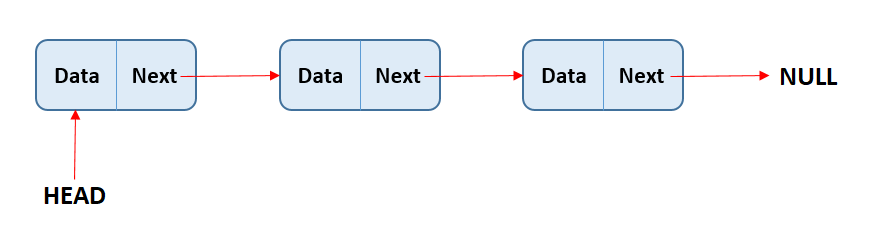
\includegraphics[width=0.8\textwidth]{aulas/aula3-lista-ligada1.png}
    \caption{Um nó}
  \end{figure}
\end{frame}

% Slide: Definição de Nó em C (Struct)
\begin{frame}[fragile]
  \frametitle{Definição de Nó em C (Struct)}
  \begin{lstlisting}[language=C]
typedef struct Node {
    int data; // Dados armazenados no nó
    struct Node* next; // Ponteiro para o próximo nó
} Node;
  \end{lstlisting}
  \begin{itemize}
    \item Esta \texttt{struct} define um nó de uma lista ligada simples em C.
    \item \texttt{data} armazena o valor do nó.
    \item \texttt{next} é um ponteiro para o próximo nó na lista, permitindo a ligação entre os nós.
  \end{itemize}
\end{frame}

% Slide: Definição de Nó em JavaScript/TypeScript
\begin{frame}[fragile]
  \frametitle{Definição de Nó em JavaScript/TypeScript}
  \begin{lstlisting}[language=JavaScript]
class Node {
    constructor(public data: number, public next: Node | null = null) {}
}
  \end{lstlisting}
  \begin{itemize}
    \item Esta classe define um nó de uma lista ligada em JavaScript/TypeScript.
    \item \texttt{data} é a propriedade que armazena o valor do nó.
    \item \texttt{next} é uma propriedade que aponta para o próximo nó na lista, inicialmente nulo se não especificado.
    \item A sintaxe \texttt{public} no construtor automaticamente declara e inicializa as propriedades da classe.
  \end{itemize}
\end{frame}

% Tipos de Listas Ligadas
% Slide: Lista Ligada Simples
\begin{frame}[fragile]
  \frametitle{Lista Ligada Simples}
  \begin{itemize}
    \item \textbf{Definição:} Uma lista ligada simples consiste em nós onde cada nó tem um ponteiro que aponta para o próximo nó na sequência.
    \item \textbf{Terminação:} O último nó aponta para NULL, indicando o fim da lista.
    \item \textbf{Operações:} Suporta operações básicas como inserção, remoção e travessia de forma eficiente, principalmente quando se trabalha no início da lista.
    \item \textbf{Uso:} Ideal para implementações simples onde a travessia é majoritariamente feita em uma única direção.
  \end{itemize}
\end{frame}

\begin{frame}[fragile]
  \frametitle{Lista ligada}
  \begin{figure}
    \centering
    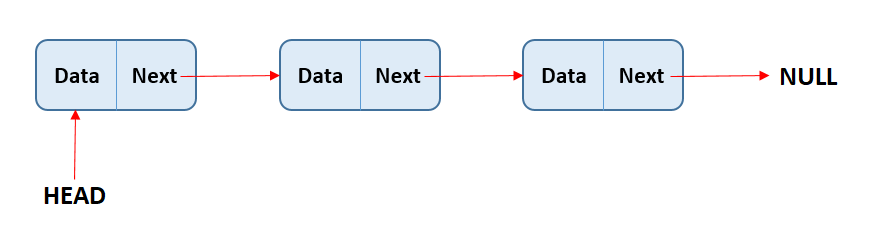
\includegraphics[width=0.8\textwidth]{aulas/aula3-lista-ligada1.png}
    \caption{Lista ligada}
  \end{figure}
\end{frame}
% Slide: Lista Duplamente Ligada
\begin{frame}[fragile]
  \frametitle{Lista Duplamente Ligada}
  \begin{itemize}
    \item \textbf{Definição:} Em uma lista duplamente ligada, cada nó contém dois ponteiros, um apontando para o próximo nó e outro para o anterior.
    \item \textbf{Flexibilidade:} Permite travessia nos dois sentidos (para frente e para trás), facilitando operações como reversão da lista e remoção de nós.
    \item \textbf{Uso de Memória:} Requer mais memória por nó em comparação com a lista ligada simples devido aos ponteiros extras.
    \item \textbf{Aplicações:} Útil em aplicações que necessitam de travessias bidirecionais ou inserções/remoções eficientes em qualquer ponto da lista.
  \end{itemize}
\end{frame}

\begin{frame}[fragile]
  \frametitle{Lista duplamente ligada}
  \begin{figure}
    \centering
    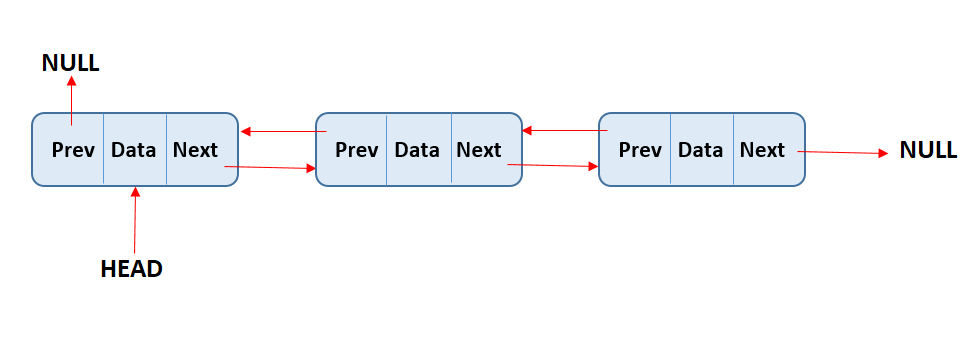
\includegraphics[width=0.8\textwidth]{aulas/aula3-dll.png}
    \caption{DLL}
  \end{figure}
\end{frame}
% Slide: Lista Circular
\begin{frame}[fragile]
  \frametitle{Lista Circular}
  \begin{itemize}
    \item \textbf{Definição:} Uma variação da lista ligada onde o último nó aponta de volta para o primeiro nó, formando um círculo.
    \item \textbf{Característica:} Não tem um fim claro como as listas ligadas simples ou duplamente ligadas, permitindo travessia contínua pela lista.
    \item \textbf{Considerações:} A implementação e a manutenção podem ser mais complexas, especialmente em listas circulares duplamente ligadas.
    \item \textbf{Uso:} Ideal para aplicações que necessitam de um ciclo contínuo de elementos, como algoritmos de round robin.
  \end{itemize}
\end{frame}

\begin{frame}[fragile]
  \frametitle{Lista circular}
  \begin{figure}
    \centering
    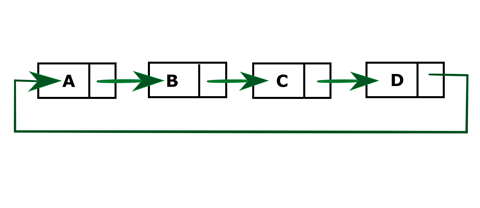
\includegraphics[width=0.8\textwidth]{aulas/aula3-cll.png}
    \caption{Lista circular}
  \end{figure}
\end{frame}

% Operações Básicas
\begin{frame}[fragile]
\frametitle{Operações Básicas}
\begin{itemize}
\item \textbf{Inserção:} Adiciona um novo nó à lista.
\begin{itemize}
\item No início, no meio, ou no fim da lista.
\end{itemize}
\item \textbf{Remoção:} Remove um nó da lista.
\begin{itemize}
\item Requer a atualização dos ponteiros do nó anterior e/ou posterior.
\end{itemize}
\item \textbf{Busca:} Encontra um nó na lista.
\begin{itemize}
\item Pode ser realizada iterando-se através dos nós até encontrar o desejado.
\end{itemize}
\item \textbf{Travessia:} Acessa cada nó da lista sequencialmente.
\end{itemize}
\end{frame}
% Slide: Inserção em Lista Ligada
\begin{frame}[fragile]
  \frametitle{Inserção em Lista Ligada}
  \begin{block}{Descrição}
    Adiciona um novo nó à lista. Pode ser realizado no início, no meio ou no fim da lista.
  \end{block}
  \small
  \begin{block}{Código em Portugol}
    procedimento inserirNoInicio(lista, valor) \\
    inicio \\
    \ \ novoNo := novo Nó \\
    \ \ novoNo.dado := valor \\
    \ \ novoNo.proximo := lista.cabeca \\
    \ \ lista.cabeca := novoNo \\
    fim
  \end{block}
\end{frame}

% Slide: Remoção em Lista Ligada
\begin{frame}[fragile]
  \frametitle{Remoção em Lista Ligada}
  \begin{block}{Descrição}
    Remove um nó da lista. Requer a atualização dos ponteiros do nó anterior (se houver) para apontar para o próximo nó do que está sendo removido.
  \end{block}
  
\end{frame}
\begin{frame}[fragile]
  \frametitle{Remoção em Lista Ligada - Código em Portugol}
  \small
  \begin{block}{Código em Portugol}
    procedimento removerNo(lista, valor) \\
    inicio \\
    \ \ se lista.cabeca = nulo então retorne fimSe \\
    \ \ se lista.cabeca.dado = valor então \\
    \ \ \ \ lista.cabeca := lista.cabeca.proximo \\
    \ \ senao \\
    \ \ \ \ atual := lista.cabeca \\
    \ \ \ \ enquanto atual.proximo ≠ nulo e atual.proximo.dado ≠ valor faça \\
    \ \ \ \ \ \ atual := atual.proximo \\
    \ \ \ \ fimEnquanto \\
    \ \ \ \ se atual.proximo ≠ nulo então \\
    \ \ \ \ \ \ atual.proximo := atual.proximo.proximo \\
    \ \ \ \ fimSe \\
    \ \ fimSe \\
    fim
  \end{block}
\end{frame}

% Slide: Busca em Lista Ligada
\begin{frame}[fragile]
  \frametitle{Busca em Lista Ligada}
  \begin{block}{Descrição}
    Encontra um nó na lista. A busca é realizada iterando-se através dos nós até encontrar o desejado.
  \end{block}
  \small
  \begin{block}{Código em Portugol}
    funcao buscarNo(lista, valor) : Nó \\
    inicio \\
    \ \ atual := lista.cabeca \\
    \ \ enquanto atual ≠ nulo faça \\
    \ \ \ \ se atual.dado = valor então \\
    \ \ \ \ \ \ retorne atual \\
    \ \ \ \ fimSe \\
    \ \ \ \ atual := atual.proximo \\
    \ \ fimEnquanto \\
    \ \ retorne nulo \\
    fim
  \end{block}
\end{frame}

% Slide: Travessia em Lista Ligada
\begin{frame}[fragile]
  \frametitle{Travessia em Lista Ligada}
  \begin{block}{Descrição}
    Acessa cada nó da lista sequencialmente. Utilizado para imprimir todos os elementos, ou para aplicar uma função a cada elemento da lista.
  \end{block}
  \small
  \begin{block}{Código em Portugol}
    procedimento percorrerLista(lista) \\
    inicio \\
    \ \ atual := lista.cabeca \\
    \ \ enquanto atual ≠ nulo faça \\
    \ \ \ \ escreva(atual.dado) \\
    \ \ \ \ atual := atual.proximo \\
    \ \ fimEnquanto \\
    fim
  \end{block}
\end{frame}

% Vantagens e Desvantagens
\begin{frame}[fragile]
\frametitle{Vantagens e Desvantagens}
\begin{itemize}
\item \textbf{Vantagens:}
\begin{itemize}
\item Flexibilidade no tamanho.
\item Inserção e remoção eficientes.
\end{itemize}
\item \textbf{Desvantagens:}
\begin{itemize}
\item Acesso sequencial (não aleatório) aos elementos.
\item Maior uso de memória devido aos ponteiros.
\end{itemize}
\end{itemize}
\end{frame}

